Il foglio di stile implementato garantisce un design fluido e scalabile, grazie all'utilizzo di unità di misura
sempre relative o in percentuale. \\Questo migliora l'accessibilità e garantisce una corretta visualizzazione delle pagine
su tutti i formati di schermi. \\Il sito dispone di 4 modalità di visualizzazione differente: desktop, tablet, mobile e di stampa.

\subsection{Desktop}
La versione desktop è stata pensata in modo avere una navigazione estremamente semplice.\\ 
Il menù, alla sinistra e molto intuitivo, rispetta la convenzione dei colori delle ancore. Infatti ogni link del menù è di colore blu, e diventa
viola nel momento in cui la pagina di destinazione è già stata visitata. \\Da notare la sottolineatura di tutti i link presenti nel sito, come convenzione.
Appunto, una persona con disabilità visive potrebbe non distinguere i link nelle pagine.\\
Nella colonna di sinistra sono presenti anche le news, con i relativi orari di apertura della pasticceria.\\ 
Da notare la larghezza massima impostata a 1200px, che permette agli utenti di utilizzare il sito con una finestra ridotta su schermi di certe dimensioni.

\begin{figure}[!h]
	\centering
	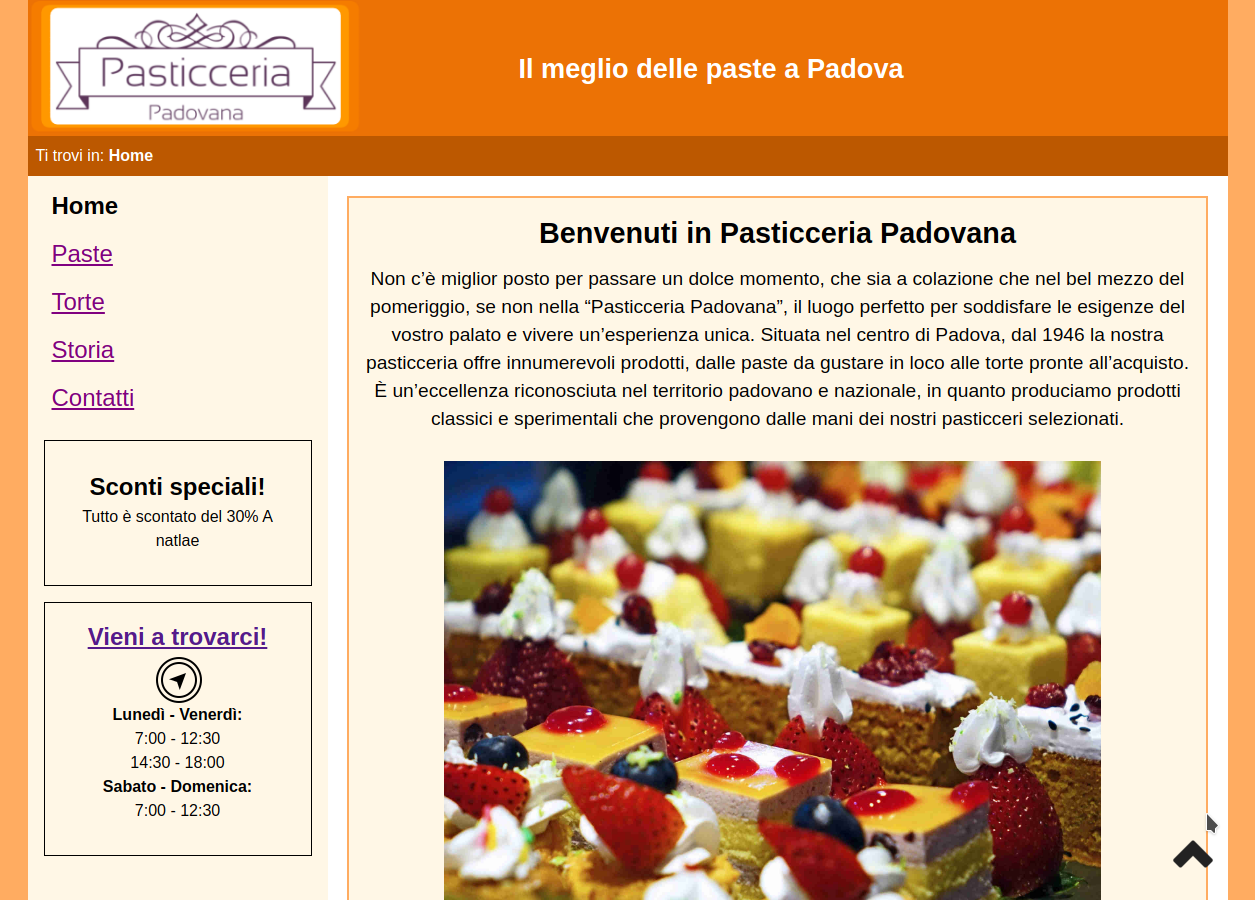
\includegraphics[width=1\linewidth]{sezioni/Progettazione/Immagini/desktop_example.png}
	\caption{Esempio di una pagina in versione desktop}
	\label{Fig:verDesktop}
\end{figure}

\subsection{Tablet}
La versione tablet implementa l'interfaccia in modo diverso. Dato lo spazio limitato dello schermo, il gruppo ha deciso di implementare
un menù ad hamburger. Anche le news non sono più laterali, ma si trovano in cima al contenuto della pagina. In questo modo viene data
maggiore importanza alle news e agli orari della pasticceria, cosa necessaria nei dispositivi portatili.\\
Anche il form di login da parte dell'amministratore nelle versioni mobili è stato nascosto e reso disponibile tramite un bottone.
\begin{figure}[!h]		
    \centering		  
	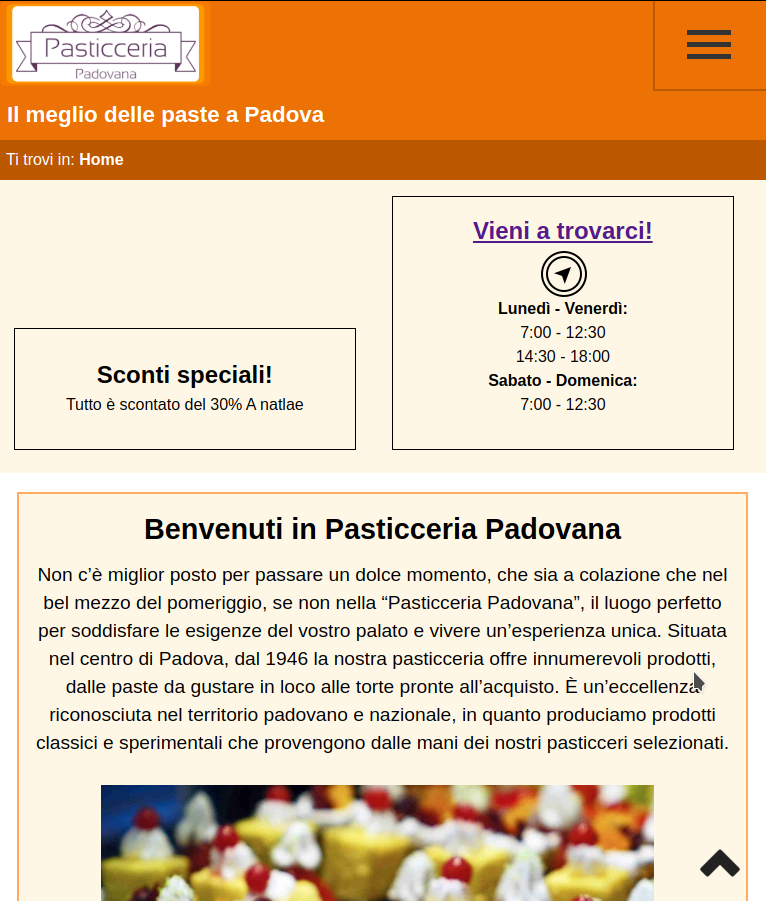
\includegraphics[width=1\linewidth]{sezioni/Progettazione/Immagini/tablet_example.png}
	\caption{Esempio di una pagina in versione tablet}
	\label{Fig:verMobile}
\end{figure}	    


\subsection{Mobile}
La versione mobile differisce di molto poco rispetto alla versione tablet. Solo le news infatti sono state allineate una sotto l'altra.
\begin{figure}[!h]
    \centering		  
	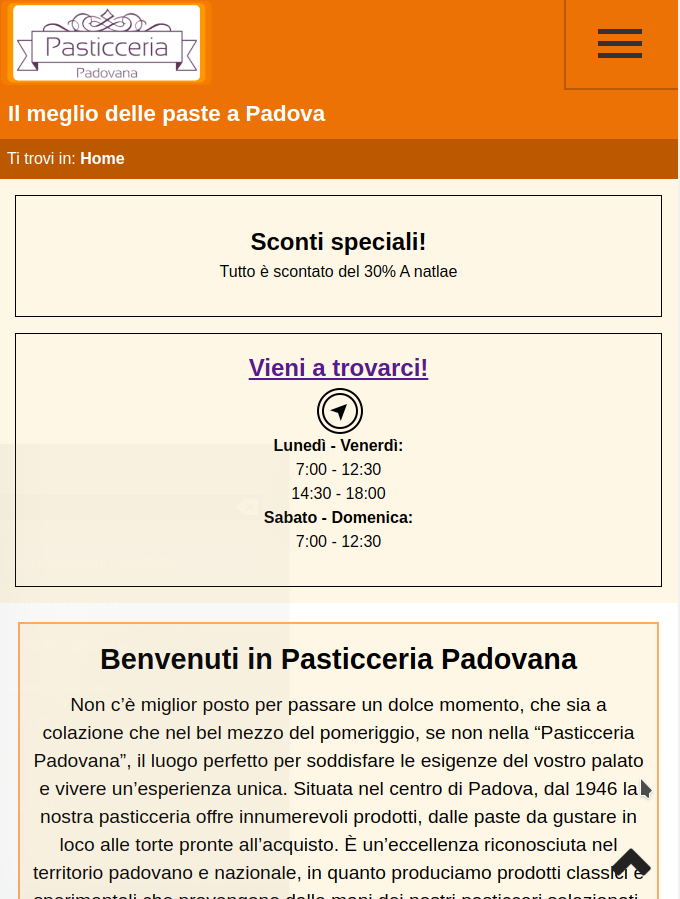
\includegraphics[width=1\linewidth]{sezioni/Progettazione/Immagini/mobile_example.png}
	\caption{Esempio di una pagina in versione mobile}
	\label{Fig:verMobile}
\end{figure}